\documentclass[DaoFP]{subfiles}
\begin{document}
\setcounter{chapter}{8}

\chapter{Natural Transformations}

We've seen that, when two objects $a$ and $b$ are isomorphic, they generate bijections between sets of arrows, which we can now express as isomorphisms between hom-sets:
\begin{align*}
\mathcal{C}(a, x) &\cong \mathcal{C}(b, x) \\
\mathcal{C}(x, a) &\cong \mathcal{C}(x, b)
\end{align*}
The converse is not true, though. An isomorphism between hom-sets does not result in an isomorphism between object \emph{unless} additional naturality conditions are satisfied. We'll now re-formulate these naturality conditions in progressively more general settings.

\section{Natural Transformations Between Hom-Functors}

One way an isomorphism between two objects can be established is by directly providing two arrows---one the inverse of the other. But quite often it's easier to do it indirectly, by defining bijections between arrows, either the ones impinging on the two objects, or the ones emanating from the two objects. 

For instance, as we've seen before, we may have, for every $x$, an invertible mapping of arrows $\alpha_x$.
\[
 \begin{tikzcd}
 \node(x) at (0, 2) {x};
 \node(a) at (-2, 0) {a};
 \node(b) at (2, 0) {b};
 \node(c1) at (-1, 1.5) {};
 \node(c2) at (-1.5, 1) {};
 \node(c3) at (-1, 2) {};
 \node(c4) at (-2, 1) {};
 \node(d1) at (1, 1.5) {};
 \node(d2) at (1.5, 1) {};
 \node(d3) at (1, 2) {};
 \node(d4) at (2, 1) {};
\node (aa) at (-1, 0.75) {};
 \node (bb) at (1, 0.75) {};
 \draw[->] (x) .. controls (c1)  and (c2) .. (a); % bend
 \draw[->, green] (x) .. controls (c3)  and (c4) .. (a); % bend
 \draw[->, blue] (x) -- (a); 
  \draw[->] (x) .. controls (d1)  and (d2) .. (b); % bend
 \draw[->, green] (x) .. controls (d3)  and (d4) .. (b); % bend
 \draw[->, blue] (x) -- (b); 
 \draw[->, red, dashed] (aa) -- node[above]{\alpha_x} (bb);
 \end{tikzcd}
\]
In other words, for every $x$, there is a mapping of hom-sets:
\[ \alpha_x \colon \mathcal{C}(x, a) \to \mathcal{C}(x, b) \]

When we vary $x$, the two hom-sets become two (contravariant) functors, $\cat C(-, a)$ and $\cat C(-, b)$, and $\alpha$ can be seen as a mapping between them. Such a mapping of functors, called a transformation, is really a family of individual mappings $\alpha_x$, one per each object $x$ in the category $\mathcal{C}$. 

The functor $\mathcal{C}(-, a)$ describes the way the worlds sees $a$, and the functor $\mathcal{C}(-, b)$ describes the way the world sees $b$. 

The transformation $\alpha$ switches back and forth between these two views. Every component of $\alpha$, the bijection $\alpha_x$, shows that the view of $a$ from $x$ is isomorphic to the view of $b$ from $x$. 

The naturality condition we discussed before was the condition:

\[ \alpha_y \circ (- \circ g) = (- \circ g) \circ \alpha_x \]
It relates components of $\alpha$ taken at different objects. In other words, it relates the views from two different observers $x$ and $y$, who are connected by the arrow $g \colon y \to x$. 

Both sides of this equation are acting on the hom-set $\mathcal{C}(x, a)$. The result is in the hom-set $\mathcal{C}(y, b)$. We can rewrite the two sides as:
\begin{align*}
 \cat C(x, a) \xrightarrow{(- \circ g)} \cat C(y, a) \xrightarrow{\alpha_y} \cat C(y, b) \\
\cat C(x, a) \xrightarrow{\alpha_x}  \cat C(x, b)  \xrightarrow{(- \circ g)}\cat C(y, b)
\end{align*}

Precomposition with $g \colon y \to x$ is also a mapping of hom-sets. In fact it is the lifting of $g$ by the contravariant hom-functor. We can write it as $\mathcal{C}(g, a)$ and $\mathcal{C}(g, b)$, respectively.
\begin{align*}
 \cat C(x, a) \xrightarrow{\cat C(g, a)} \cat C(y, a) \xrightarrow{\alpha_y} \cat C(y, b) \\
\cat C(x, a) \xrightarrow{\alpha_x}  \cat C(x, b)  \xrightarrow{\cat C(g, b)}\cat C(y, b)
\end{align*}

The naturality condition can therefore be rewritten as:
\[ \alpha_y \circ \mathcal{C}(g, a) = \mathcal{C}(g, b) \circ \alpha_x \]
It can be illustrated by this commuting diagram:
\[
 \begin{tikzcd}
 \mathcal{C}(x, a)
 \arrow[d, "\alpha_x"]
 \arrow[r, "{\mathcal{C}(g, a)}"]
 &
 \mathcal{C}(y, a)
  \arrow[d, "\alpha_y"]
 \\
 \mathcal{C}(x, b)
 \arrow[r, "{\mathcal{C}(g, b)}"]
& \mathcal{C}(y, b)
 \end{tikzcd}
\]

We can now say that  an invertible transformation $\alpha$ between the functors $\mathcal{C}(-, a)$ and $\mathcal{C}(-, b)$ that satisfies the naturality condition is equivalent to an isomorphism between $a$ and $b$.

We can follow exactly the same reasoning for the outgoing arrows. This time we start with a transformation $\beta$ whose components are:
\[ \beta_x \colon \mathcal{C}(a, x) \to \mathcal{C}(b, x) \]
The two (covariant) functors $\mathcal{C}(a, -)$ and $\mathcal{C}(b, -)$ describe the view of the world from the perspective of $a$ and $b$, respectively. The invertible transformation $\beta$ tells us that these two views are equivalent, and the naturality condition 
\[ (g \circ -) \circ \beta_x = \beta_y \circ (g \circ -) \]
tells us that they behave nicely when we switch focus.

Here's the commuting diagram that illustrates the naturality condition:
\[
 \begin{tikzcd}
 \mathcal{C}(a, x)
 \arrow[d, "\beta_x"]
 \arrow[r, "{\mathcal{C}(a, g)}"]
 &
 \mathcal{C}(a, y)
  \arrow[d, "\beta_y"]
 \\
 \mathcal{C}(b, x)
 \arrow[r, "{\mathcal{C}(b, g)}"]
& \mathcal{C}(b, y)
 \end{tikzcd}
\]

Again, such an invertible natural transformation $\beta$ establishes the isomorphism between $a$ and $b$.

\section{Natural Transformation Between Functors}

The two hom-functors from the previous section were
\begin{align*}
 F x &=   \mathcal{C}(a, x) \\
G x &=   \mathcal{C}(b, x)
\end{align*}
They both map the category $\mathcal{C}$ to  $\mathbf{Set}$, because that's where the hom-sets live. We can say that they create two different \emph{models} of $\mathcal{C}$ inside $\mathbf{Set}$. 

A natural transformation is a structure-preserving mapping between such models. 
\[
 \begin{tikzcd}
 && \cat C(a, x)
 \arrow[dd, "\beta_x"]
 \\
 x
 \arrow[rru, dashed, "{\cat C(a, -)}"]
 \arrow[rrd, dashed, "{\cat C(b, -)}"']
 \\
 && \cat C(b, x)
 \end{tikzcd}
\]


This idea naturally extends to functors between any pair of categories. Any two functors
\begin{align*}
F &\colon \mathcal{C} \to \mathcal{D} \\
G &\colon \mathcal{C} \to \mathcal{D}
\end{align*}
may be seen as two different models of $\mathcal{C}$ inside $\mathcal{D}$. 

To transform one model into another we connect the corresponding dots using arrows in $\mathcal{D}$. For every object $x$ in $\mathcal{C}$ we pick an arrow that goes from $F x$ to $G x$:
\[ \alpha_x \colon F x \to G x \]
A natural transformation thus maps objects to arrows.
\[
 \begin{tikzcd}
 && F x
 \arrow[dd, "\alpha_x"]
 \\
 x
 \arrow[rru, dashed, "F"]
 \arrow[rrd, dashed, "G"']
 \\
 && G x
 \end{tikzcd}
\]


The structure of a model, though, has as much to do with objects as it does with arrows, so let's see what happens to arrows. For every arrow $f \colon x \to y$ in $\mathcal{C}$, we have two corresponding arrows in $\mathcal{D}$:
\begin{align*}
 F f &\colon F x \to F y \\
G f &\colon G x \to G y 
\end{align*}
These are the two liftings of $f$. You can use them to move within the bounds of each of the two models. Then there are the components of $\alpha$ which let you switch between models. 

Naturality says that it shouldn't matter whether you first move inside the first model and then jump to the second one, or first jump to the second one and then move within it. This is illustrated by the commuting \emph{naturality square}:

\[
 \begin{tikzcd}
 F x
 \arrow[d, "\alpha_x"]
 \arrow[r, "F f"]
 &
F y
  \arrow[d, "\alpha_y"]
 \\
G x
 \arrow[r, "G f"]
& G y
 \end{tikzcd}
\]

Such a family of arrows $\alpha_x$ that satisfies the naturality condition is called a \emph{natural transformation}.

This is a diagram that shows a pair of categories, two functors between them, and a natural transformation $\alpha$ between the functors:
\[
\begin{tikzcd}[column sep=huge]
\mathcal{C}
  \arrow[bend left=50]{r}[name=U, label=above:$F$]{}
  \arrow[bend right=50]{r}[name=D, label=below:$G$]{} 
 &
\mathcal{D}
  \arrow[shorten <=10pt,shorten >=10pt,Rightarrow,to path={(U) -- node[label=left:$\alpha$] {} (D)}]{}
\end{tikzcd}
\]


Since for every arrow in $\mathcal{C}$ there is a corresponding naturality square, we can say that a natural transformation maps objects to arrows, and arrows to commuting squares.

If every component $\alpha_x$ of a natural transformation is an isomorphism, $\alpha$ is called a \emph{natural isomorphism}. 

We can now restate the main result about isomorphisms: Two objects are isomorphic if and only if there is a natural isomorphism between their hom-functors (either the covariant, or the contravariant ones---either one will do).

Natural transformations provide a very convenient high-level way of expressing commuting conditions in a variety of situations. We'll use them in this capacity to reformulate the definitions of algebraic data types.

\section{Natural Transformations in Programming}

A natural transformation is a family of arrows parameterized by objects. In programming, this corresponds to a family of functions parameterized by types, that is a \emph{polymorphic function}. 

The type of the argument to a natural transformation is described using one functor, and the return type using another. 

In Haskell, we can define a data type that accepts two type constructors representing two functors, and produces a type of natural transformations:

\begin{haskell}
data Natural :: (Type -> Type) -> (Type -> Type) -> Type where
  Natural :: (forall a. f a -> g a) -> Natural f g
\end{haskell}
The \hask{forall} quantifier tells the compiler that the function is polymorphic---that is, it's defined for every type \hask{a}. As long as \hask{f} and \hask{g} are functors, this formula defines a natural transformation. 

The types defined by \hask{forall} are very special, though. The are polymorphic in the sense of \index{parametric polymorphism}\emph{parametric polymorphism}. It means that a single formula is used for all types. We've seen the example of the identity function, which can be written as:
\begin{haskell}
id :: forall a. a -> a
id x = x
\end{haskell}
The body of this function is very simple, just the variable \hask{x}. It doesn't matter what type \hask{x} is, the formula remains the same.

This is in contrast to \index{ad-hoc polymorphism}\emph{ad-hoc polymorphism}. An ad-hoc polymorphic function may use different implementations for different types. An example of such a function is \hask{fmap}, the member function of the \hask{Functor} typeclass. There is one implementation of \hask{fmap} for lists, a different one for \hask{Maybe}, and so on, case by case. 

The standard definition of a (parametric) natural transformation in Haskell uses a \emph{type synonym:}
\begin{haskell}
type Natural f g = forall a. f a -> g a
\end{haskell}
A \index{\hask{type} synonym}\hask{type} declaration introduces an alias, a shorthand, for the right-hand-side.

It turns out that limiting the type of a natural transformation to adhere to parametric polymorphism has far reaching consequences. Such a function automatically satisfies naturality conditions. It's an example of \index{parametricity}parametricity producing so called \index{theorems for free}\emph{theorems for free}. 

We can't express equalities of arrows in Haskell, but we can use naturality to transform programs. In particular, if \hask{alpha} is a natural transformation, we can replace:
\begin{haskell}
fmap h . alpha
\end{haskell}
with:
\begin{haskell}
alpha . fmap h
\end{haskell}
Here, the compiler will automatically figure out what versions of \hask{fmap} and which components of \hask{alpha} to use. 

We can also use more advanced language options to make the choices explicit. We can express naturality using a pair of functions: 
\begin{haskell}
oneWay :: 
  forall f g a b. (Functor f, Functor g) => 
  Natural f g -> (a -> b) -> f a -> g b
oneWay alpha h = fmap @g h . alpha @a
\end{haskell}
\begin{haskell}
otherWay :: 
  forall f g a b. (Functor f, Functor g) => 
  Natural f g -> (a -> b) -> f a -> g b
otherWay alpha h = alpha @b . fmap @f h
\end{haskell}
The annotations \hask{@a} and \hask{@b} specify the components of the parametrically polymorphic function \hask{alpha}, and the annotations \hask{@f} and \hask{@g} specify the functors for which the ad-hoc polymorphic \hask{fmap} is instantiated.

The following Haskell extensions have to be specified at the top of the file:
\begin{haskell}
{-# language RankNTypes #-}
{-# language TypeApplications #-}
{-# language ScopedTypeVariables #-}
\end{haskell}

Here's an example of a useful function that is a natural transformation between the list functor and the \hask{Maybe} functor:
\begin{haskell}
safeHead :: Natural [] Maybe
safeHead [] = Nothing
safeHead (a : as) = Just a
\end{haskell}
(The standard library \hask{head} function is ``unsafe'' in that it faults when given an empty list.)

Another example is the function \hask{reverse}, which reverses a list. It's a natural transformation from the list functor to the list functor:
\begin{haskell}
reverse :: Natural [] []
reverse [] = []
reverse (a : as) = reverse as ++ [a]
\end{haskell}
Incidentally, this is a very inefficient implementation. The actual library function uses an optimized algorithm.

A useful intuition for understanding natural transformations builds on the idea that functors acts like containers for data. There are two completely orthogonal things that you can do with a container: You can transform the data it contains, without changing the shape of the container. This is what \hask{fmap} does. Or you can transfer the data, without modifying it, to another container. This is what a natural transformation does: It's a procedure for moving ``stuff'' between containers without knowing what kind of ``stuff'' it is. 

In other words, a natural transformations repackages the contents of one container into another container. It does it in a way that is agnostic of the type of the contents, which means it cannot inspect, create, or modify this contents. All it can do is to move it to a new location, or drop it. 

Naturality condition enforces the orthogonality of these two operations. It doesn't matter if you first modify the data and then move it to another container; or first move it, and then modify. 

This is another example of successfully decomposing a complex problem into a sequence of simpler ones. Keep in mind, though, that not every operation with containers of data can be decomposed in that way. Filtering, for instance, requires both examining the data, as well as changing the size or even the shape of the container. 

On the other hand, almost every parametrically polymorphic function is a natural transformation. In some cases you may have to consider the identity or the constant functor as either source or the target. For instance, the polymorphic identity function can be though of as a natural transformation between two identity functors.

\subsection{Vertical composition of natural transformations}

Natural transformations can only be defined between \emph{parallel} functors, that is functors that share the same source category and the same target category. Such parallel functors form a \emph{functor category}. The standard notation for a functor category between two categories $\mathcal{C}$ and $\mathcal{D}$ is $[\mathcal{C}, \mathcal{D}]$, that is the names of the two categories between square brackets.

The objects in $[\mathcal{C}, \mathcal{D}]$ are functors, the arrows are natural transformations. 

To show that this is indeed a category, we have to define the composition of natural transformations. This is easy if we keep in mind that components of natural transformations are regular arrows in the target category. These arrows compose.

Indeed, suppose that we have a natural transformation $\alpha$ between two functors $F$ and $G$. We want to compose it with another natural transformation $\beta$ that goes from $G$ to $H$. 

\[
\begin{tikzcd}[column sep=huge]
\mathcal{C}
  \arrow[bend left=60]{rr}[name=U, label=above:$F$]{}
  \arrow[]{rr}[name=M, label={[xshift=15pt, yshift=-5pt]:$G$}]{} 
  \arrow[bend right=60]{rr}[name=D, label=below:$H$]{} 
 &&
\mathcal{D}
  \arrow[shorten <=8pt, shorten >=8pt,Rightarrow, to path={(U) -- node[label=left:$\alpha$] {} (M)}]{}
  \arrow[shorten <=8pt, shorten >=8pt,Rightarrow, to path={(M) -- node[label=left:$\beta$] {} (D)}]{}
\end{tikzcd}
\]


Let's look at the components of these transformations at some object $x$
\[ \alpha_x \colon F \, x \to G \, x \]
\[ \beta_x \colon G \, x \to H \, x \]
These are just two arrows in $\mathcal{D}$ that are composable. So we can define a composite natural transformation $\gamma$ as follows:
\[ \gamma \colon F \to H\]
\[ \gamma_x = \beta_x \circ \alpha_x \]
 This is called the \emph{vertical composition} of natural transformations. You'll see it written using a dot $\gamma = \beta \cdot \alpha$ or a simple juxtaposition $\gamma = \beta \alpha$.
 
Naturality condition for $\gamma$ can be shown by pasting together (vertically) two naturality squares for $\alpha$ and $\beta$:
\[
 \begin{tikzcd}
 F x
 \arrow[d, "\alpha_x"]
 \arrow[r, "F f"]
 \arrow[dd, bend right = 60, "\gamma_x"']
 &
F y
  \arrow[d, "\alpha_y"]
 \arrow[dd, bend left = 60, "\gamma_y"]
 \\
G x
 \arrow[r, "G f"]
 \arrow[d, "\beta_x"]
& G y
\arrow[d, "\beta_y"]
\\
H x
\arrow[r, "H f"]
& H y
 \end{tikzcd}
\]

In Haskell, vertical composition of natural transformation is just regular function composition applied to polymorphic functions. Using the intuition that natural transformations move items between containers, vertical composition combines two such moves, one after another.

\subsection{Functor categories}

Since the composition of natural transformations is defined in terms of composition of arrows, it is automatically associative. 

There is also an identity natural transformation $id_F$ defined for every functor $F$. Its component at $x$ is the usual identity arrow at the object $F x$:
\[ (id_F)_x = id_{F x} \]

To summarize, for every pair of categories $\mathcal{C}$ and $\mathcal{D}$ there is a category of functors $[\mathcal{C}, \mathcal{D}]$ with natural transformations as arrows. 

The hom-set in that category is the set of natural transformations between two functors $F$ and $G$. Following the standard notational convention, we write it as:
\[ [\mathcal{C}, \mathcal{D}](F, G) \]
with the name of the category followed by the names of the two objects (here, functors) in parentheses.

In category theory objects and arrows are drawn differently. Objects are dots and arrows are pointy lines.

In $\mathbf{Cat}$, the category of categories, functors are drawn as arrows. But in a functor category $[\cat C, \cat D]$ functors are dots and natural transformations are arrows.

What is an arrow in one category could be an object in another.


\begin{exercise}
Prove the naturality condition of the composition of natural transformations:
\[ \gamma_y \circ F f = H f \circ \gamma_x \]
Hint: Use the definition of $\gamma$ and the two naturality conditions for $\alpha$ and $\beta$.
\end{exercise}


\subsection{Horizontal composition of natural transformations}

The second kind of composition of natural transformations is induced by composition of functors. Suppose that we have a pair of composable functors
\begin{align*}
 F \colon \mathcal{C} \to \mathcal{D}
&&G \colon \mathcal{D} \to \mathcal{E} 
\end{align*}
and, in parallel, another pair of composable functors:
\begin{align*}
 F' \colon \mathcal{C} \to \mathcal{D}
&& G' \colon \mathcal{D} \to \mathcal{E} 
\end{align*}
We also have two natural transformations:
\begin{align*}
\alpha \colon F \to F'  
&& \beta \colon G \to G' 
\end{align*}
Pictorially:
\[
\begin{tikzcd}[column sep=huge]
\mathcal{C}
  \arrow[bend left=50]{r}[name=U, label=above:$F$]{}
  \arrow[bend right=50]{r}[name=D, label=below:$F'$]{} 
 &
\mathcal{D}
  \arrow[bend left=50]{r}[name=U1, label=above:$G$]{}
  \arrow[bend right=50]{r}[name=D1, label=below:$G'$]{} 
 &
\mathcal{E}
  \arrow[shorten <=10pt,shorten >=10pt,Rightarrow,to path={(U) -- node[label=left:$\alpha$] {} (D)}]{}
  \arrow[shorten <=10pt,shorten >=10pt,Rightarrow,to path={(U1) -- node[label=left:$\beta$] {} (D1)}]{}
\end{tikzcd}
\]
The \emph{horizontal composition} $\beta \circ \alpha$ maps $G \circ F$ to $G' \circ F'$.

Let's pick an object $x$ in $\mathcal{C}$ and try to define the component of the composite $(\beta \circ \alpha)$ at $x$. It should be a morphism in $\cat E$:
\[ (\beta \circ \alpha)_x \colon G ( F x) \to G' ( F' x) \]

We can use $\alpha$ to map $x$ to an arrow 
\[ \alpha_x \colon F x \to F' x \]
We can lift this arrow using $G$
\[ G (\alpha_x) \colon G (F x) \to G (F' x) \]
To get from there to $G' (F' x)$ we can use the appropriate component of $\beta$
\[ \beta_{F' x} \colon G (F' x) \to G' (F' x) \]
Altogether, we have
\[ (\beta \circ \alpha)_x = \beta_{F' x} \circ G (\alpha_x) \]

But there is another equally plausible candidate: 
\[ (\beta \circ \alpha)_x = G'(\alpha_x) \circ \beta_{F x}\]
Fortunately, the are equal due to naturality of $\beta$. 

\[
 \begin{tikzcd}
  && G(F x)
  \arrow[dd, red, "G(\alpha_x)"]
  \arrow[dr, blue, "\beta_{F x}"]
  \\
  & F x
  \arrow[rr, bend right=10, dashed, gray]
  \arrow[ur, bend right=10, dashed]
  \arrow[dd, red, "\alpha_x"]
 && G' (F x)
  \arrow[dd, red, "G'(\alpha_x)"]
 \\
 x
 \arrow[ur, dashed]
 \arrow[dr, gray, dashed]
 && G(F' x)
  \arrow[dr, blue, "\beta_{F' x}"]
 \\
 &F' x
  \arrow[rr, bend right=10, dashed, gray]
 \arrow[ur, bend right=10, dashed]
 && G'(F' x)
\end{tikzcd}
\]
The proof of naturality of $\beta \circ \alpha$ is left as an exercise to a dedicated reader.

We can translate this directly to Haskell. We start with two natural transformations:
\begin{haskell}
alpha :: forall x. F x -> F' x
beta  :: forall x. G x -> G' x
\end{haskell}
Their horizontal composition has the following type signature:
\begin{haskell}
beta_alpha :: forall x. G (F x) -> G' (F' x)
\end{haskell}
It has two equivalent implementations. The first one is:
\begin{haskell}
beta_alpha = beta . fmap alpha
\end{haskell}
The compiler will automatically pick the correct version of \hask{fmap}, the one for the functor \hask{G}. The second implementation is:
\begin{haskell}
beta_alpha = fmap alpha . beta
\end{haskell}
Here, the compiler will pick the version of \hask{fmap} for the functor \hask{G'}.

What's the intuition for horizontal composition? We've seen before that a natural transformation can be seen as repackaging data between two containers--functors. Here we are dealing with nested containers. We start with the outer container described by \hask{G} that is filled with inner containers, each described by \hask{F}. We have two natural transformations, \hask{alpha} for transfering the contents of \hask{F} to \hask{F'}, and \hask{beta} for moving the contents of \hask{G} to \hask{G'}. There are two ways of moving data from \hask{G (F x)} to \hask{G'(F' x)}. We can use \hask{fmap alpha} to repackage all inner containers, and then use \hask{beta} to repackage the outer container. 

\[
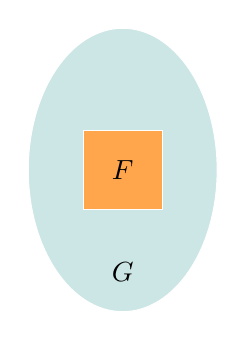
\begin{tikzpicture}
\filldraw[fill=blue!50!green!20, draw=white] (0, 0) ellipse (1.2 and 1.8);
\filldraw[fill=orange!70, draw=white] (-0.5, -0.5) rectangle (0.5, 0.5);
\node at (0, 0) {$F$};
\node at (0, -1.3) {$G$};
\end{tikzpicture}
\hspace{20pt}
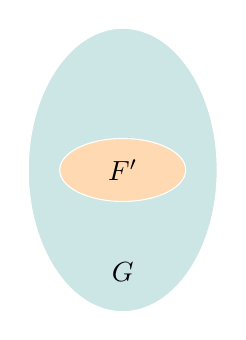
\begin{tikzpicture}
\filldraw[fill=blue!50!green!20, draw=white] (0, 0) ellipse (1.2 and 1.8);
\filldraw[fill=orange!30, draw=white] (0, 0) ellipse (0.8 and 0.4);
\node at (0, 0) {$F'$};
\node at (0, -1.3) {$G$};
\end{tikzpicture}
\hspace{20pt}
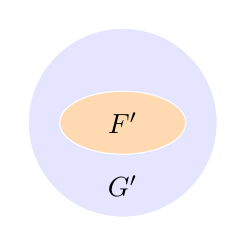
\begin{tikzpicture}
\filldraw[fill=blue!10, draw=white] (0, 0) circle (1.2);
\filldraw[fill=orange!30, draw=white] (0, 0) ellipse (0.8 and 0.4);
\node at (0, 0) {$F'$};
\node at (0, -0.8) {$G'$};
\end{tikzpicture}
\]


Or we can first use \hask{beta} to repackage the outer container, and then apply \hask{fmap alpha} to repackage all the inner containers. The end result is the same.

\[
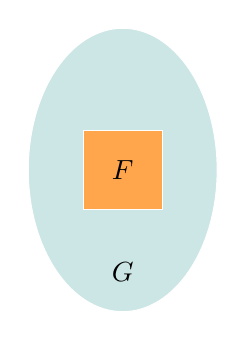
\begin{tikzpicture}
\filldraw[fill=blue!50!green!20, draw=white] (0, 0) ellipse (1.2 and 1.8);
\filldraw[fill=orange!70, draw=white] (-0.5, -0.5) rectangle (0.5, 0.5);
\node at (0, 0) {$F$};
\node at (0, -1.3) {$G$};
\end{tikzpicture}
\hspace{20pt}
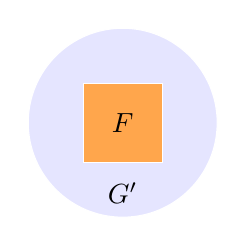
\begin{tikzpicture}
\filldraw[fill=blue!10, draw=white] (0, 0) circle (1.2);
\filldraw[fill=orange!70, draw=white] (-0.5, -0.5) rectangle (0.5, 0.5);
\node at (0, 0) {$F$};
\node at (0, -0.9) {$G'$};
\end{tikzpicture}
\hspace{20pt}
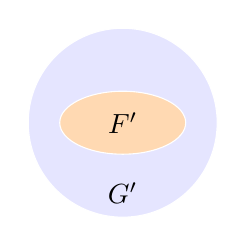
\begin{tikzpicture}
\filldraw[fill=blue!10, draw=white] (0, 0) circle (1.2);
\filldraw[fill=orange!30, draw=white] (0, 0) ellipse (0.8 and 0.4);
\node at (0, 0) {$F'$};
\node at (0, -0.9) {$G'$};
\end{tikzpicture}
\]


\begin{exercise}
Implement two versions of horizontal composition of \hask{safeHead} after \hask{reverse}. Compare their results acting on various arguments.
\end{exercise}

\begin{exercise}
Do the same with the horizontal composition of \hask{reverse} after \hask{safeHead}. 
\end{exercise}

\subsection{Whiskering}

Quite often horizontal composition is used with one of the natural transformations being the identity. There is a shorthand notation for such composition. For instance, $\alpha \circ id_F$ is written as $\alpha \circ F$. 

Because of the characteristic shape of the diagram, such composition is called ``whiskering''.
\[
\begin{tikzcd}[column sep=huge]
\mathcal{C}
 \arrow[r, "F"]
 &
\mathcal{D}
  \arrow[bend left=50]{r}[name=U1, label=above:$G$]{}
  \arrow[bend right=50]{r}[name=D1, label=below:$G'$]{} 
 &
\mathcal{E}
  \arrow[shorten <=10pt,shorten >=10pt,Rightarrow,to path={(U1) -- node[label=left:$\alpha$] {} (D1)}]{}
\end{tikzcd}
\]
In components, we have:
\[ (\alpha \circ F)_x = \alpha_{F x} \]

Let's consider how we would translate this to Haskell. A natural transformation is a polymorphic function. Because of parametricity, it's defined by the same formula for all types. So whiskering on the right doesn't change the formula, it changes function signature. 

For instance, if this is the declaration of \hask{alpha}:
\begin{haskell}
alpha :: forall x. G x -> G' x
\end{haskell}
then its whiskered version would be:
\begin{haskell}
alpha_f :: forall x. G (F x) -> G' (F x)
alpha_f = alpha
\end{haskell}
Because of Haskell's type inference, this shift is implicit. When a polymorphic function is called, we don't have to specify which component of the natural transformation is executed--the type checker figures it out by looking at the type of the argument. 

The intuition in this case is that we are repackaging the outer container leaving the inner containers intact.

Similarly, $id_H \circ \alpha$ is written as $H \circ \alpha$.
\[
\begin{tikzcd}[column sep=huge]
\mathcal{D}
  \arrow[bend left=50]{r}[name=U, label=above:$G$]{}
  \arrow[bend right=50]{r}[name=D, label=below:$G'$]{} 
 &
\mathcal{E}
\arrow[r, "H"]
&
\mathcal{F}
  \arrow[shorten <=10pt,shorten >=10pt,Rightarrow,to path={(U) -- node[label=left:$\alpha$] {} (D)}]{}
\end{tikzcd}
\]
In components:
\[(H \circ \alpha)_x = H (\alpha_x) \]

In Haskell, the lifting of $\alpha_x$ by $H$ is done using \hask{fmap}, so given:
\begin{haskell}
alpha :: forall x. G x -> G' x
\end{haskell}
the whiskered version would be:
\begin{haskell}
h_alpha :: forall x. H (G x) -> H (G' x)
h_alpha = fmap alpha
\end{haskell}
Again, Haskell's type inference engine figures out which version of \hask{fmap} to use (here, it's the one from the \hask{Functor} instance of \hask{G}).

The intuition is that we are repackaging the contents of the inner containers leaving the outer container intact.

Finally, in many applications a natural transformation is whiskered on both sides:
\[
\begin{tikzcd}[column sep=huge]
\mathcal{C}
 \arrow[r, "F"]
 &
\mathcal{D}
  \arrow[bend left=50]{r}[name=U1, label=above:$G$]{}
  \arrow[bend right=50]{r}[name=D1, label=below:$G'$]{} 
 &
\mathcal{E}
  \arrow[shorten <=10pt,shorten >=10pt,Rightarrow,to path={(U1) -- node[label=left:$\alpha$] {} (D1)}]{}
  \arrow[r, "H"]
 &
 \mathcal{F}
\end{tikzcd}
\]
In components, we have:
\[ (H \circ \alpha \circ F) x = H (\alpha_{F x})\]
and in Haskell:
\begin{haskell}
h_alpha_f :: forall x. H (G (F x)) -> H (G' (F x))
h_alpha_f = fmap alpha
\end{haskell}

Here the intuition is that we have a triple layer of containers; and we are rearranging the middle one, leaving the outer container and all the inner containers intact.

\subsection{Interchange law}

We can combine vertical composition with horizontal composition, as seen in the following diagram:
\[
\begin{tikzcd}[column sep=huge]
\mathcal{C}
  \arrow[bend left=60]{rr}[name=U, label=above:$F$]{}
  \arrow[]{rr}[name=M, label={[xshift=15pt, yshift=-5pt]:$G$}]{} 
  \arrow[bend right=60]{rr}[name=D, label=below:$H$]{} 
 &&
\mathcal{D}
  \arrow[bend left=60]{rr}[name=U1, label=above:$F'$]{}
  \arrow[]{rr}[name=M1, label={[xshift=15pt, yshift=-5pt]:$G'$}]{} 
  \arrow[bend right=60]{rr}[name=D1, label=below:$H'$]{} 
&&
\mathcal{E}
  \arrow[shorten <=8pt, shorten >=8pt,Rightarrow, to path={(U) -- node[label=left:$\alpha$] {} (M)}]{}
  \arrow[shorten <=8pt, shorten >=8pt,Rightarrow, to path={(M) -- node[label=left:$\beta$] {} (D)}]{}
  \arrow[shorten <=8pt, shorten >=8pt,Rightarrow, to path={(U1) -- node[label=left:$\alpha'$] {} (M1)}]{}
  \arrow[shorten <=8pt, shorten >=8pt,Rightarrow, to path={(M1) -- node[label=left:$\beta'$] {} (D1)}]{}
\end{tikzcd}
\]
The interchange law states that the order of composition doesn't matter: we can first do vertical compositions and then the horizontal one, or first do the horizontal compositions and then the vertical one.


\section{Universal Constructions Revisited}

Lao Tzu says, the simplest pattern is the clearest.

We've seen definitions of sums, products, exponentials, natural numbers, and lists. 

The old-school approach to defining such data types is to explore their internals. It's the set-theory way: we look at how the elements of new sets are constructed from the elements of old sets. An element of a sum is either an element of the first set, or the second set. An element of a product is a pair of elements. And so on. We are looking at objects from the engineering point of view.

In category theory we take the opposite approach. We are not interested in what's inside the object or how it's implemented. We are interested in the purpose of the object, how it can be used, and how it interacts with other objects. We are looking at objects from the utilitarian point of view.

Both approaches have their advantages. The categorical approach came later, because you need to study a lot of examples before clear patterns emerge. But once you see the patterns, you discover unexpected connections between things, like the duality between sums and products.

Defining particular objects through their connections requires looking at possibly infinite numbers of objects with which they interact. 

``Tell me your relation to the Universe, and I'll tell you who you are.''

Defining an object by its mappings-out or mappings-in with respect to all objects in the category is called a \emph{universal construction}. 

Why are natural transformations so important? It's because most categorical constructions involve commuting diagrams. If we can re-cast these diagrams as naturality squares, we move one level up the abstraction ladder and gain new valuable insights.

Being able to compress a lot of facts into small elegant formulas helps us see new patterns. We'll see, for instance, that natural isomorphisms between hom-sets pop up all over category theory and eventually lead to the idea of an adjunction.

But first we'll study several examples in greater detail to get some understanding of the terse language of category theory. We'll try, for instance, to decode the statement that the sum, or the coproduct of two objects, is defined by the following natural isomorphism:

\[ [\mathbf{2}, \mathcal{C}](D, \Delta_x)  \cong \mathcal{C}(a + b, x) \]



\subsection{Picking objects}

Even such a simple task as pointing at an object has a special interpretation in category theory. We have already seen that pointing at an element of a set is equivalent to selecting a function from the singleton set to it. Similarly, picking an object in a category is equivalent to selecting a functor from the single-object category. Or it can be done using a constant functor from another category. 

Quite often we want to pick a pair of objects. That, too, can be accomplished by selecting a functor from a two-object stick-figure category. Similarly, picking an arrow is equivalent to selecting a functor from the ``walking arrow'' category, and so on.

By judiciously selecting our functors and natural transformations between them, we can reformulate all the universal constructions we've seen so far.

\subsection{Cospans as natural transformations}

The definition of a sum requires the selection of two objects to be summed; and a third one to serve as the target of the mapping out.

\[
 \begin{tikzcd}
 a
 \arrow[dr,  bend left, "\text{Left}"']
 \arrow[ddr, bend right, "f"']
 && b
 \arrow[dl, bend right, "\text{Right}"]
 \arrow[ddl, bend left, "g"]
 \\
&a + b
\arrow[d, dashed, "h"]
\\
& c
 \end{tikzcd}
\]
This diagram can be further decomposed into two simpler shapes called \emph{cospans}:
\[
 \begin{tikzcd}
 a
 \arrow[dr, ""']
 && b
 \arrow[dl, ""]
 \\
 & x
 \end{tikzcd}
\]

To construct a cospan we first have to pick a pair of objects. To do that we'll start with a two-object category $\mathbf{2}$. We'll call its objects $1$ and $2$. 
We'll use a functor 
\[ D \colon \mathbf{2} \to \mathcal{C}\]
to select the objects $a$ and $b$: 
\begin{align*}
D\, 1 &= a \\
D\, 2 &= b 
\end{align*}
($D$ stands for ``diagram'', since the two objects form a very simple diagram consisting of two dots in $\mathcal{C}$.)

We'll use the constant functor 
\[ \Delta_x \colon \mathbf{2} \to \mathcal{C} \]
to select the object $x$. This functor maps both $1$ and $2$ to $x$ (and the two identity arrows to $id_x$).

Since both functors go from $\mathbf{2}$ to $\mathcal{C}$, we can define a natural transformation $\alpha$ between them. In this case, it's just a pair of arrows:
\begin{align*}
\alpha_1 \colon D \, 1 \to \Delta_x 1 \\
\alpha_2 \colon D \, 2 \to \Delta_x 2
\end{align*}
These are exactly the two arrows in the cospan. 

Naturality condition for $\alpha$ is trivial, since there are no arrows (other than identities) in $\mathbf{2}$.

There may be many cospans sharing the same three objects---meaning: there may be many natural transformations between the two functors $D$ and  $\Delta_x$. These natural transformations form a hom-set in the functor category $[\mathbf{2}, \mathcal{C}]$, namely:
\[ [\mathbf{2}, \mathcal{C}](D, \Delta_x) \]

\subsection{Functoriality of cospans}

Let's consider what happens when we start varying the object $x$ in a cospan. We have a mapping $F$ that takes $x$ to the set of cospans over $x$:
\[ F x = [\mathbf{2}, \mathcal{C}](D, \Delta_x) \]
This mapping turns out to be functorial in $x$.

To see that, consider an arrow $m \colon x \to y$. The lifting of this arrow is a mapping between two sets of natural transformations:
\[ [\mathbf{2}, \mathcal{C}](D, \Delta_x) \to [\mathbf{2}, \mathcal{C}](D, \Delta_{y}) \] 
 
This might look very abstract until you remember that natural transformations have components, and these components are just regular arrows. An element of the left-hand side is a natural transformation:
\[ \mu \colon D \to \Delta_x \]
It has two components corresponding to the two objects in $\mathbf{2}$. For instance, we have
\[ \mu_1 \colon D \, 1 \to \Delta_x 1 \]
or, using the definitions of $D$ and $\Delta$:
\[ \mu_1 \colon a \to x \]
This is just the left leg of our cospan. 

Similarly, the element of the right-hand side is a natural transformation:
\[ \nu \colon D \to \Delta_{y} \]
Its component at $1$ is an arrow
\[ \nu_1 \colon a \to y \]
We can get from $\mu_1$ to $\nu_1$ simply by post-composing it with $m \colon x \to y$. So the lifting of $m$ is a component-by-component post-compositon $(m \circ -)$:
\begin{align*}
\nu_1 = m \circ \mu_1 \\
\nu_2 = m \circ \mu_2 \\
\end{align*}

\subsection{Sum as a universal cospan}

Of all the cospans that you can build on the pair $a$ and $b$, the one with the arrows we called $\text{Left}$ and $\text{Right}$ converging on $a + b$  is very special. There is a unique mapping out of it to any other cospan---a mapping that makes two triangles commute.  
\[
 \begin{tikzcd}
 a
 \arrow[dr,  bend left, "\text{Left}"']
 \arrow[ddr, bend right, "f"']
 && b
 \arrow[dl, bend right, "\text{Right}"]
 \arrow[ddl, bend left, "g"]
 \\
&a + b
\arrow[d, dashed, "h"]
\\
& x
 \end{tikzcd}
\]

We are now in a position to translate this condition to a statement about natural transformations and hom-sets. The arrow $h$ is an element of the hom-set 
\[ \mathcal{C}(a + b, x)\]
A cospan over $x$ is a natural transformation, that is an element of the hom-set in the functor category:
\[ [\mathbf{2}, \mathcal{C}](D, \Delta_x) \]

Both are hom-sets in their respective categories. And both are just sets, that is objects in the category $\mathbf{Set}$. This category forms a bridge between the functor category $[\mathbf{2}, \mathcal{C}]$ and a ``regular'' category $\mathcal{C}$, even though, conceptually, they seem to be at very different levels of abstraction. 

Paraphrasing Sigmund Freud, ``Sometimes a set is just a set.''

Our universal construction is the bijection or the isomorphism of sets:
\[ [\mathbf{2}, \mathcal{C}](D, \Delta_x)  \cong \mathcal{C}(a + b, x) \]

Moreover, if we vary the object $x$, the two sides behave like functors from  $\mathcal{C}$ to $\mathbf{Set}$. Therefore it makes sense to ask if this mapping of functors is a natural isomorphism. 

Indeed, it can be shown that the naturality condition for this isomorphism translates into commuting conditions for the triangles in the definition of the sum. So the definition of the sum can be replaced by a single equation.

\subsection{Product as a universal span}

An analogous argument can be made about the universal construction for the product. Again, we start with the stick-figure category $\mathbf{2}$ and the functor $D$. But this time we use a natural transformation going in the opposite direction
\[ \alpha \colon \Delta_x \to D \]
Such a natural transformation is a pair of arrows that form a \emph{span}:
\[
 \begin{tikzcd}
 &x
 \arrow[dl, "f"']
 \arrow[dr, "g"]
 \\
 a
 && b
  \end{tikzcd}
\]
Collectively, these natural transformations form a hom-set in the functor category :
\[[\mathbf{2}, \mathcal{C}](\Delta_x, D) \]

Every element of this hom-set is in one-to-one correspondence with a unique mapping $h$ into the product $a \times b$. Such a mapping is a member of the hom-set $\mathcal{C}(x, a \times b)$. This correspondence is expressed as the isomorphism:
\[ [\mathbf{2}, \mathcal{C}](\Delta_x, D)  \cong \mathcal{C}(x, a \times b) \]
It can be shown that the naturality of this isomorphism guarantees that the triangles in this diagram commute:
\[
 \begin{tikzcd}
 & C 
\arrow[d, dashed, "h"]
 \arrow[ddl, bend right, "f = \alpha_1"']
 \arrow[ddr, bend left, "g = \alpha_2"]
\\
&a \times b
 \arrow[dl,  "\text{fst}"]
  \arrow[dr,   "\text{snd}"']
\\
a = D\, 1 && b = D \, 2
 \end{tikzcd}
\]

\subsection{Exponentials}

The exponentials, or function objects, are defined by this commuting diagram:
\[
 \begin{tikzcd}
 x \times a
 \arrow[d, dashed, "h \times id_a"']
 \arrow[rd, "f"]
 \\
 b^a \times a
 \arrow[r, "\varepsilon_{a b}"']
& b
 \end{tikzcd}
\]
Here, $f$ is an element of the hom-set $\mathcal{C}(x \times a, b)$ and $h$ is an element of $\mathcal{C}(x, b^a)$. 

The isomorphism between these sets, natural in $x$, defines the exponential object. 
\[\mathcal{C}(x \times a, b) \cong \mathcal{C}(x, b^a)\]

The $f$ in the diagram above is an element of the left-hand side, and $h$ is the corresponding element of the right-hand side. The transformation $\alpha_x$ (which also depends on $a$ and $b$) maps $f$ to $h$.
\[ \alpha_x \colon \mathcal{C}(x \times a, b) \to \mathcal{C}(x, b^a) \]
In Haskell, we call it \hask{curry}. Its inverse, $\alpha^{-1}$ is known as \hask{uncurry}.

Unlike in the previous examples, here both hom-sets are in the same category, and it's easy to analyze the isomorphism in more detail. In particular, we'd like to see how the commuting condition:
\[  f = \varepsilon_{a b} \circ (h \times id_a) \]
arises from naturality.

The standard Yoneda trick is to make a substitution for $x$ that would reduce one of the hom-sets to an endo-hom-set, that is a hom-set whose source is the same the target. This will allow us to pick a canonical element of that hom-set, that is the identity arrow.

In our case, substituting $b^a$ for $x$ will allow us to pick $h = id_{(b^a)}$.
\[
 \begin{tikzcd}
 b^a \times a
 \arrow[d, dashed, "id_{(b^a)} \times id_a"']
 \arrow[rd, "f"]
 \\
 b^a \times a
 \arrow[r, "\varepsilon_{a b}"']
& b
 \end{tikzcd}
\]
The commuting condition in this case tells us that $f = \varepsilon_{a b}$. In other words, we get the formula for $\varepsilon_{a b}$ in terms of $\alpha$:
\[ \varepsilon_{a b} = \alpha_{x}^{-1} (id_{x}) \]
where $x$ is equal to $b^a$.

Since we recognize $\alpha^{-1}$ as \hask{uncurry}, and $\varepsilon$ as function application, we can write it in Haskell as:
\begin{haskell}
apply :: (a -> b, a) -> b
apply = uncurry id
\end{haskell}
This my be surprising at first, until you realize that the currying of \hask{(a->b,a)->b} leads to \hask{(a->b)->(a->b)}.

We can also encode the two sides of the main isomorphism as Haskell functors:
\begin{haskell}
data LeftFunctor  a b x = LF ((x, a) -> b)
\end{haskell}
\begin{haskell}
data RightFunctor a b x = RF (x -> (a -> b))
\end{haskell}
They are both contravariant functors in the type variable \hask{x}.
\begin{haskell}
instance Contravariant (LeftFunctor a b) where
  contramap g (LF f) = LF (f . bimap g id)
\end{haskell}
This says that the lifting of $g \colon x \to y$ is given by the following pre-composition:
\[ \mathcal{C}(y \times a, b) \xrightarrow{(- \circ (g \times id_a)) }  \mathcal{C}(x \times a, b)\]

Similarly:
\begin{haskell}
instance Contravariant (RightFunctor a b) where
  contramap g (RF h) = RF (h . g)
\end{haskell}
translates to:
\[  \mathcal{C}(y, b^a) \xrightarrow{ (- \circ g) } \mathcal{C}(x, b^a) \]

The natural transformation $\alpha$ is just a thin encapsulation of \hask{curry}; and its inverse is \hask{uncurry}:

\begin{haskell}
alpha :: forall a b x. LeftFunctor a b x -> RightFunctor a b x
alpha (LF f) = RF (curry f)
\end{haskell}

\begin{haskell}
alpha_1 :: forall a b x. RightFunctor a b x -> LeftFunctor a b x
alpha_1 (RF h) = LF (uncurry h)
\end{haskell}

Using the two formulas for the lifting of $g \colon x \to y$, here's the naturality square:

\[
 \begin{tikzcd}
 \mathcal{C}(y \times a, b)
 \arrow[rr, "(- \circ (g \times id_a))"]
 \arrow[d,  "\alpha_y"]
& &
\mathcal{C}(x \times a, b)
  \arrow[d, "\alpha_x"]
 \\
 \mathcal{C}(y, b^a)
 \arrow[rr, "(- \circ g)"]
& &
\mathcal{C}(x, b^a)
 \end{tikzcd}
\]

Let's now apply the Yoneda trick to it and replace $y$ with $b^a$. This also allows us to substitute $g$---which now goes for $x$ to $b^a$---with $h$. 

\[
 \begin{tikzcd}
 \mathcal{C}(b^a \times a, b)
 \arrow[rr, "(- \circ (h \times id_a))"]
 \arrow[d,  "\alpha_{(b^a)}"]
& &
\mathcal{C}(x \times a, b)
  \arrow[d,  "\alpha_x"]
 \\
 \mathcal{C}(b^a, b^a)
 \arrow[rr, "(- \circ h)"]
& &
\mathcal{C}(x, b^a)
 \end{tikzcd}
\]

We know that the hom-set $\mathcal{C}(b^a, b^a)$ contains at least the identity arrow, so we can pick the element $id_{(b^a)}$ in the lower left corner. 

Reversing the arrow on the left, we know that $\alpha^{-1}$ acting on identity produces $\varepsilon_{a b}$ in the upper left corner (that's the \hask{uncurry id} trick). 

Pre-composition with $h$ acting on identity produces $h$ in the lower right corner. 

$\alpha^{-1}$ acting on $h$ produces $f$ in the upper right corner. 

\[
 \begin{tikzcd}[
  every arrow/.style={draw,mapsto}
]
 \varepsilon_{a b}
 \arrow[rr, "(- \circ (h \times id_a))"]
& &
f
 \\
 id_{(b^a)}
 \arrow[u, "\alpha^{-1}"]
 \arrow[rr, "(- \circ h)"]
& &
h
\arrow[u, "\alpha^{-1}"']
 \end{tikzcd}
\]
(The $\mapsto$ arrows denote the action of functions on elements of sets.)


So the selection of $id_{(b^a)}$ in the lower left corner fixes the other three corners. In particular, we can see that the upper arrow applied to $\varepsilon_{a b}$ produces $f$, which is exactly the commuting condition:
\[ \varepsilon_{a b} \circ (h \times id_a) = f \]
the one that we set out to derive.

\section{Limits and Colimits}

In the previous section we defined the sum and the product using natural transformations. These were transformations between diagrams defined as functors from a very simple stick-figure category $\mathbf{2}$, one of the functors being the constant functor. 

Nothing prevents us from replacing the category $\mathbf{2}$ with something more complex. For instance, we could try categories that have non-trivial arrows between objects, or categories with infinitely many objects. 

There is a whole vocabulary built around such constructions. 

We used objects in the category $\mathbf{2}$ for indexing objects in the category $\mathcal{C}$. We can replace $\mathbf{2}$ with an arbitrary indexing category $\cat J$. A diagram in $\mathcal{C}$ is still defined as a functor $D \colon \cat J \to \mathcal{C}$. It picks objects in $\mathcal{C}$, but it also picks some arrows between them.

As the second functor we'll still use the constant functor $\Delta_x \colon \cat J \to \mathcal{C}$.

A  natural transformation, that is an element of the hom-set
\[ [\cat J, \mathcal{C}](\Delta_x, D)  \]
is now called a \emph{cone}. Its dual, an element of
\[ [\cat J, \mathcal{C}](D, \Delta_x)  \]
is called a \emph{cocone}. They generalize the span and the cospan, respectively.

Diagramatically, cones and cocones look like this:
\[
 \begin{tikzcd}
  & x
\arrow[ddr, "g"]
 \arrow[ddl, "f"']
 \arrow[ddd, "h"]
 \\
\\
D 1 
\arrow[rr, red]
\arrow[rd, red]
&& D 2
\arrow[dl, red]
\\
& D 3
 \end{tikzcd}
 \qquad
\begin{tikzcd}
 D 1
 \arrow[rr, red]
 \arrow[dr, red]
 \arrow[dddr, "f"']
 && D 2
\arrow[dl, red]
 \arrow[dddl, "g"]
 \\
 & D 3
 \arrow[dd, "h"]
 \\
 \\
 & x
 \end{tikzcd}
 \]

Since the indexing category may now contain arrows, the naturality conditions for these diagrams are no longer trivial. The constant functor $\Delta_x$ shrinks all vertices to one, so naturality squares shrink to triangles. Naturality means that all triangles with $x$ in their apex must now commute. 

The universal cone, if it exists, is called the \emph{limit} of the diagram $D$, and is written as $\text{Lim}D$. Universality means that it satisfies the following isomorphism, natural in $x$:
\[ [\cat J, \mathcal{C}](\Delta_x, D)  \cong \mathcal{C}(x, \text{Lim}D) \]

A limit of a $\Set$-valued functor has a particularly simple characterization. It's a set of cones with the singleton set at the apex. Indeed, elements of the limit, that is functions from the singleton set to it, are in one-to-one correspondence with such cones:
\[ [\cat J, \mathcal{C}](\Delta_1, D)  \cong \mathcal{C}(1, \text{Lim}D) \]


Dually, the universal cocone is called a \emph{colimit}, and is described by the following natural isomorphism:
\[ [\cat J, \mathcal{C}](D, \Delta_x)  \cong \mathcal{C}( \text{Colim}D, x) \]


We can now say that a product is a limit (and a sum is a colimit) of a diagram from the indexing category $\mathbf{2}$.

Limits and colimits distill the essence of a pattern. 

A limit, like a product, is defined by its mapping-in property. A colimit, like a sum, is defined by its mapping-out property.

There are many interesting limits and colimits, and we'll see some when we discuss algebras and coalgebras.

\begin{exercise}
Show that the limit of a ``walking arrow'' category, that is a two-object category with an arrow connecting the two objects, has the same elements as the first object in the diagram (``elements'' are the arrows from the terminal object).
\end{exercise}

\subsection{Equalizers}

A lot of high-school math involves learning how to solve equations or systems of equations. An equation equates the outcomes of two different ways of producing something. If we are allowed to subtract things, we usually shove everything to one side and simplify the problem to calculating the zeros of some expression. In geometry, the same idea is expressed as the intersection of two geometric objects.

In category theory all these patterns are embodied in a single construction called an equalizer. An equalizer is a limit of a diagram whose pattern is given by a stick-figure category with two parallel arrows:
\[
\begin{tikzcd}
i \arrow[r, shift left=0.75ex]
  \arrow[r, shift right=0.75ex]
&
j
\end{tikzcd}
\]
The two arrows represent two ways of producing something. 

A functor from this category picks a pair of objects and a pair of morphisms in the target category. The limit of this diagram embodies an intersection of the two outcomes. It is an object $e$ with two arrows $p \colon e \to a$ and $p' \colon e \to b$.
\[
\begin{tikzcd}
& e
\arrow[dl, "p"']
\arrow[dr, gray, "p'"]
\\
a 
\arrow[rr, red, shift left=.75ex, "f"]
\arrow[rr, red, shift right=.75ex, "g"']
&&
b
\end{tikzcd}
\]
We have two commuting conditions:
\begin{align*}
p' &= f \circ h \\
p' &= g \circ h
\end{align*}
It means that $p'$ is fully determined by one of the equations, while the other turns into the constraints:
\[ f \circ p = g \circ p \]
Since the equalizer is the limit, it is the universal such pair, as illustrated in this diagram:
\[
\begin{tikzcd}
x
\arrow[d, dashed, "h"']
\arrow[dr, ""]
\\
e
\arrow[r, "p"']
&
a \arrow[r, red, shift left=0.75ex, "f"]
  \arrow[r, red, shift right=0.75ex, "g"']
&
b
\end{tikzcd}
\]

To develop the intuition for equalizers it's instructive to consider how it works for sets. As usual, the trick is to replace $x$ with the singleton set $1$:
\[
\begin{tikzcd}
1
\arrow[d, dashed, "e"']
\arrow[dr, "a"]
\\
E
\arrow[r, "p"']
&
A \arrow[r, red, shift left=0.75ex, "f"]
  \arrow[r, red, shift right=0.75ex, "g"']
&
B
\end{tikzcd}
\]
In this case $a$ is an element of $A$ such that $f a = g a$. That's just a way of saying that $a$ is the solution of a pair of equations. Universality means that there is a unique element $e$ of $E$ such that $p \circ e = a$. In other words, elements of $E$ are in one-to-one correspondence with the solutions of the system of equations. 

\subsection{Coequalizers}

What's dual to equating or intersecting? It's the process of discovering commonalities and organizing things into buckets. For instance, we can distribute integers into even and odd buckets. In category theory, this process of bucketizing is described by coequalizers.

A coequalizer is the colimit of the same diagram that we used to define the equalizer:
\[
\begin{tikzcd}
a 
\arrow[rr, red, shift left=.75ex, "f"]
\arrow[rr, red, shift right=.75ex, "g"']
\arrow[rd, gray, "q'"']
&&
b
\arrow[ld, "q"]
\\
& c
\end{tikzcd}
\]
This time, the arrow $q'$ is fully determined by $q$; and $q$ must satisfy the equation:
\[ q \circ f = q \circ g \]

Again, we can gain some intuition by considering a coequalizer of two functions acting on sets. 
\[
\begin{tikzcd}
A
\arrow[r, red, shift left=.75ex, "f"]
\arrow[r, red, shift right=.75ex, "g"']
&
B
\arrow[r, "q"]
& C
\end{tikzcd}
\]
An $x \in A$ is mapped to two elements $f x$ and $g x$ in $B$, but then $q$ maps them back to a single element of $C$. This element represents the bucket. Universality means that $C$ is a copy of $B$ in which the elements that were produced from the same $x$ have been identified.

Consider an example where $A$ is a set of pairs of integers \hask{(m, n)}, such that either both are even or both are odd.  We want to coequalize two functions that are the two projections \hask{(fst, snd)}. The equalizer set $C$ will have two elements corresponding to two buckets. We'll represent it as \hask{Bool}. The equalizing function \hask{q} selects the bucket:
\begin{haskell}
q :: Int -> Bool
q n = n `mod` 2 == 0 
\end{haskell}
Any function \hask{q'} that cannot distinguish between the components of our pairs can be uniquely factorized through the function \hask{h}:
\begin{haskell}
h :: (Int -> a) -> Bool -> a
h q' True  = g' 0
h q' False = g' 1
\end{haskell}

\begin{exercise}
Run a few tests that show that, in the example above, the factorization \hask{(h g') . q} gives the same result as \hask{g'} given by the following definition:
\begin{haskell}
import Data.Bits

q' :: Int -> Bool
q' x = testBit x 0
\end{haskell}

\end{exercise}
\begin{exercise}
What is the coequalizer of the pair \hask{(id, reverse)}, both of the type \hask{String->String}? Test its universality by factorizing the following function:
\begin{haskell}
q' :: String -> Maybe Char
q' s = if even len
       then Nothing
       else Just (s !! (len `div` 2))
  where len = length s
\end{haskell}
\end{exercise}

\subsection{The existence of the terminal object}

Lao Tzu says: great acts are made up of small deeds.

So far we've been studying limits of tiny diagrams, that is functors from simple stick-figure categories. Nothing, however, prevents us from defining limits and colimits where the patterns are taken to be infinite categories. But there is a gradation of infinities. When the objects in a category form a proper set, we call such a category  \index{small category}\emph{small}. Unfortunately, the very basic example, the category $\Set$ of sets, is not small. We know that there is no set of all sets. $\Set$ is a \index{large category}\emph{large} category. But at least all the hom-sets in $\Set$ are sets. We say that $\Set$ is \index{locally small category}\emph{locally small}. In what follows we'll be always working with locally small categories.

A small limit is a limit of a small diagram, that is a functor from a category whose objects and morphisms form sets. A category in which all small limits exist is called small complete, or just \emph{complete}. In particular, in such a category, a product of an arbitrary \emph{set} of objects exists. You can also equalize an arbitrary set of arrows between two objects. If such category is locally small, that means all equalizers exist.

Conversely, a (small) cocomplete category has all small colimits. In particular, such a category has all small coproducts and coequalizers.

The category $\Set$ is both complete and cocomplete. 


In a cocomplete locally small category there is a simple criterion for the existence of the terminal object: It's enough that a weakly terminal set exists. 

A \index{weakly terminal object}\emph{weakly terminal} object, just like the terminal object, has an arrow coming from any object; except that such an arrow is not necessarily unique. 

A \index{weakly terminal set}\emph{weakly terminal set} is a family of objects $t_i$ indexed by a set $I$ such that, for any object $c$ in $\cat C$ there exists an $i$ and an arrow $c \to t_i$. Such a set is also called a \index{solution set}\emph{solution set}.

\[
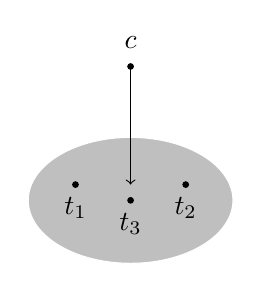
\begin{tikzpicture}
        \filldraw (0, 1.5) circle (1pt);
        \node at (0, 1.8) {$c$};
        
\filldraw[fill=gray!50, draw=white] (0, -0.2) ellipse (1.3 and 0.8);
        \filldraw (-0.7, 0) circle (1pt);
        \node at (-0.7, -0.3) {$t_1$};
        \filldraw (0.7, 0) circle (1pt);
        \node at (0.7, -0.3) {$t_2$};
        \filldraw (0, -0.2) circle (1pt);
        \node at (0, -0.5) {$t_3$};
        
    	\draw[->] (0, 1.5) -- (0, 0);
\end{tikzpicture}
\]

In a cocomplete category we can always construct a coproduct $\coprod_{i \in I} t_i$. This coproduct is a weakly terminal object, because there is an arrow to it from every $c$. This arrow is the composite of the arrow to some $t_i$ followed by the injection $\iota_i \colon t_i \to \coprod_{j \in I} t_j$.

Given a weakly terminal object, we can construct the (strongly) terminal object. We first define a subcategory $\cat T$ of $\cat C$ whose objects are $t_i$. Morphisms in $\cat T$ are all the morphisms in $\cat C$ that go between the objects of $\cat T$. This is called a \index{full subcategory}\emph{full} subcategory of $\cat C$. By our construction, $\cat T$ is small.

There is an obvious inclusion functor $F$ that embeds $\cat T$ in $\cat C$. This functor defines a small diagram in $\cat C$. It turns out that the colimit of this diagram is the terminal object in $\cat C$.

Dually, a similar construction can be used to define an initial object as a limit of a weakly initial set.

This property of solution sets will come handy in the proof of the Freyd's adjoint functor theorem.

\section{The Yoneda Lemma}

A functor from some category $\mathcal{C}$ to the category of sets can be thought of as a model of this category in $\mathbf{Set}$. Modeling, in general, is a lossy process: it discards some information. A constant $\Set$-valued functor is an extreme example: it maps the whole category to a single set and its identity function. 

A hom-functor produces a model of the category as viewed from a certain vantage point. The functor $\mathcal{C}(a, -)$, for instance, offers the panorama of $\mathcal{C}$ from the vantage point of $a$. It organizes all the arrows emanating from $a$ into neat packages that are connected by images of arrows that go between them, all in accordance with the original structure of the source category. 

\[
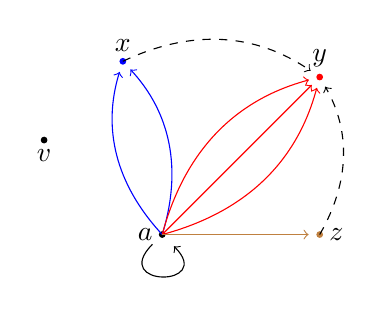
\begin{tikzpicture}
\def\ax{0}
\def\ay{0.5}
\def\xx{-0.5}
\def\xy{2.7}
\def\yx{2}
\def\yy{2.5}
\def\zx{2}
\def\zy{0.5}
\def\vx{-1.5}
\def\vy{1.7}
\filldraw[black] (\ax, \ay) circle (1 pt);
\node (a) at (\ax, \ay) {};
\node[left] at (\ax, \ay) {$a$};
\filldraw[blue] (\xx, \xy) circle (1 pt);
\node[above] at (\xx, \xy) {$x$};
\filldraw[red] (\yx, \yy) circle (1 pt);
\node[above] at (\yx, \yy) {$y$};
\filldraw[brown] (\zx, \zy) circle (1 pt);
\node[right] at (\zx, \zy) {$z$};
\filldraw[black] (\vx, \vy) circle (1 pt);
\node[below] at (\vx, \vy) {$v$};

\draw [->] (a) edge[out=225, in=315, loop] (a);

\draw[dashed] (\xx, \xy) edge[->, bend left, shorten > = 4 pt] (\yx, \yy);
\draw[dashed] (\zx, \zy) edge[->, bend right, shorten > = 4 pt] (\yx, \yy);

\draw[blue] (\ax, \ay) edge[->, bend left, shorten > = 4 pt] (\xx, \xy);
\draw[blue] (\ax, \ay) edge[->, bend right, shorten > = 4 pt] (\xx, \xy);

\draw[red] (\ax, \ay) edge[->, bend left, shorten > = 4 pt] (\yx, \yy);
\draw[red] (\ax, \ay) edge[->, bend right, shorten > = 4 pt] (\yx, \yy);
\draw[red] (\ax, \ay) edge[->, shorten > = 4 pt] (\yx, \yy);

\draw[brown] (\ax, \ay) edge[->, shorten > = 4 pt] (\zx, \zy);
\end{tikzpicture}
\hspace{80pt}
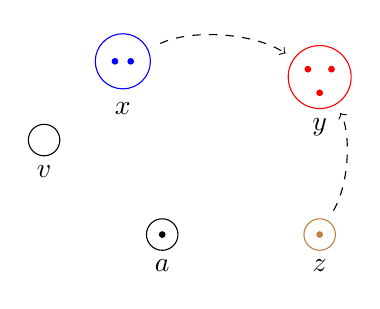
\begin{tikzpicture}
\def\ax{0}
\def\ay{0.5}
\def\xx{-0.5}
\def\xy{2.7}
\def\yx{2}
\def\yy{2.5}
\def\zx{2}
\def\zy{0.5}
\def\vx{-1.5}
\def\vy{1.7}
\def\sx{0.7}
\def\sy{1.6}

\node at (\sx, \sy) {$\Set$};

\draw[black] (\vx, \vy) circle (0.2);
\node[below] at (\vx, \vy - 0.2) {$v$};

\draw[black] (\ax, \ay) circle (0.2);
\filldraw[black] (\ax, \ay) circle (1 pt);
\node[below] at (\ax, \ay-0.2) {$a$};

\draw[blue] (\xx, \xy) circle (0.35);
\filldraw[blue] (\xx - 0.1, \xy) circle (1 pt);
\filldraw[blue] (\xx + 0.1, \xy) circle (1 pt);
\node[above] at (\xx, \xy - 0.8) {$x$};

\draw[red] (\yx, \yy) circle (0.4);
\filldraw[red] (\yx-0.15, \yy+0.1) circle (1 pt);
\filldraw[red] (\yx+0.15, \yy+0.1) circle (1 pt);
\filldraw[red] (\yx, \yy-0.2) circle (1 pt);
\node[below] at (\yx, \yy - 0.4) {$y$};

\draw[brown] (\zx, \zy) circle (0.2);
\filldraw[brown] (\zx, \zy) circle (1 pt);
\node[below] at (\zx, \zy - 0.2) {$z$};

\draw[dashed] (\xx, \xy) edge[->, bend left, shorten > = 15, shorten < = 15] (\yx, \yy);
\draw[dashed] (\zx, \zy) edge[->, bend right, shorten > = 15, shorten < = 10] (\yx, \yy);

\end{tikzpicture}
\]


Some vantage points are better than others. For instance, the view from the initial object is quite sparse. Every object $x$ is mapped to a singleton set $\cat C(0, x)$ corresponding to the unique mapping $0 \to x$. 

The view from the terminal object is more interesting: it maps all objects to their sets of (global) elements $\cat C(1, x)$. 

The Yoneda lemma may be considered one of the most profound statements, or one of the most trivial statements in category theory. Let's start with the profound version. 

Consider two models of $\mathcal{C}$ in $\mathbf{Set}$: one given by the hom-functor  $\mathcal{C}(a, -)$, that is the panoramic view of $\mathcal{C}$ from the vantage point of $a$; and another given by some arbitrary functor $F \colon \mathcal{C} \to \mathbf{Set}$. A natural transformation between them embeds one model in the other. It turns out that the set of such natural transformations is fully determined by the value of $F$ at $a$.

The set of natural transformation is the hom-set in the functor category $[\mathcal{C}, \mathbf{Set}]$, so this is the formal statement of the Yoneda lemma:

\[ [\mathcal{C}, \mathbf{Set}]( \mathcal{C}(a, -), F) \cong F a \]

The reason this works is because all the mappings involved in this theorem are bound by the requirements of preserving the structure of the category $\mathcal{C}$ and the structure of its models. In particular, naturality conditions impose a huge set of constraints on the way the components of a natural transformation propagate from one point to another. 

The proof of the Yoneda lemma starts with a single identity arrow and lets naturality propagate it across the whole category.

Here's the sketch of the proof. It consists of two parts: First, given a natural transformation we construct an element of $F a$. Second, given an element of $F a$ we construct the corresponding natural transformation. 

First, let's pick an arbitrary element on the left-hand side: a natural transformation $\alpha$. Its component at $x$ is a function:
\[ \alpha_x \colon \mathcal{C}(a, x) \to F x \]
We can now apply the Yoneda trick: substitute $a$ for $x$:
\[ \alpha_a \colon \mathcal{C}(a, a) \to F a \]
and then pick the identity $id_a$ as the canonical element of $\mathcal{C}(a, a)$. This gives us an element $\alpha_a (id_a)$ in the set $F a$. This defines a mapping in one direction, from natural transformations to elements of the set $F a$.

Looking at the picture of the hom-functor $\cat C(a, -)$, we notice that its action on $a$ itself is always a non-empty set. If there is a natural transformation from it to $F$, it means that $F a$ must be non-empty too.
\[
\begin{tikzpicture}
\def\ax{0}
\def\ay{0.5}
\def\xx{-0.5}
\def\xy{3.7}
\filldraw[black] (\ax, \ay) circle (1 pt);
\node (a) at (\ax, \ay) {};
\node[left] at (\ax, \ay) {$a$};
\filldraw[blue] (\xx, \xy) circle (1 pt);
\node[above] at (\xx, \xy) {$x$};

\draw [->] (a) edge[out=225, in=315, loop] (a);
\node[right] at (\ax + 0.3, \ay - 0.35) {$id_a$};

\draw[blue] (\ax, \ay) edge[->, "$h$", bend right, shorten > = 4 pt] (\xx, \xy);

\end{tikzpicture}
\hspace{80pt}
\begin{tikzpicture}

\def\ax{0}
\def\ay{0.5}
\def\xx{-0.5}
\def\xy{3.7}

\def\fax{3}
\def\fay{0.5}
\def\fxx{3 - 0.5}
\def\fxy{3.7}

\def\px{\fax - 0.3}
\def\hx{\xx + 0.35}
% C(a,a)
\draw[black] (\ax, \ay) circle (0.2);
\filldraw[black] (\ax, \ay) circle (1 pt);
\node[below] at (\ax, \ay-0.2) {$\cat C (a, a)$};
% C(a,x)
\draw[black] (\xx, \xy) ellipse (0.7 and 0.4);

\filldraw[blue] (\xx + 0.35, \xy) circle (1 pt);
\node[left, blue] at (\hx, \xy) {$h$};

\node[above] at (\xx, \xy - 1.1) {$\cat C (a, x)$};
\draw[dashed] (\hx, \xy) edge[->, "$\alpha_x$", shorten > = 4 pt] (\fxx, \fxy);

% F a
\draw[red] (\fax, \fay) ellipse (0.7 and 0.4);
\filldraw[red] (\px, \fay) circle (1 pt);
\node[right, red] at (\px, \fay) {$p$};
\node[right, red] at (\fax + 0.7, \fay) {$F a$};
\draw[dashed] (\ax, \ay) edge[->, "$\alpha_a$", shorten > = 3 pt] (\px, \fay);
% F x
\draw[red] (\fxx, \fxy) circle (0.4);
\filldraw[red] (\fxx, \fxy) circle (1 pt);
\node[right, red] at (\fxx + 0.35, \fxy) {$F x$};

\draw[blue] (\px, \fay) edge[->, "$F h$", bend right, shorten > = 12, shorten < = 12] (\fxx, \fxy);

\end{tikzpicture}
\]


Now the other way around. Given an element $p$ of the set $F a$ we want to construct a natural transformation $\alpha$. First, we pick $p$ to be the action of $\alpha_a$ on $id_a \in \cat C(a, a)$. 

Now let's take an arbitrary object $x$ and an arbitrary element of $\cat C(a, x)$. Such an element corresponds to some arrow $h \colon a \to x$. Our natural transformation must map it to an element of $F x$. We can do it by lifting the arrow $h$ using $F$. We get a function:
\[F h \colon F a \to F x \]
We can apply this function to $p$ and get an element of $F x$. We take this element as the action of $\alpha_x$ on $h$:
\[ \alpha_x h = (F h) p \]

The isomorphism in the Yoneda lemma is natural not only in $a$ but also in $F$. In other words, you can ``move'' from the functor $F$ to another functor $G$ by applying an arrow in the functor category, that is a natural transformation. This is quite a leap in the levels of abstraction, but all the definitions of functoriality and naturality work equally well in the functor category, where objects are functors, and arrows are natural transformations.

\begin{exercise}
Fill in the gap in the proof when $F a$ is empty.
\end{exercise}
\begin{exercise}
Show that the mapping 
\[ \mathcal{C}(a, x) \to F x\]
defined above is a natural transformation. Hint: Vary $x$ using some $f \colon x \to y$.
\end{exercise}
\begin{exercise}
Show that the formula for $\alpha_x$ can be derived from the assumption that $\alpha_a (id_a) = p$ and the naturality condition. Hint: The lifting of $h$ by the hom-functor $\cat C(a, h)$ is given by post-composition.
\end{exercise}

\subsection{Yoneda lemma in programming}

Now for the trivial part: The proof of the Yoneda lemma translates directly to Haskell code. We start with the type of natural transformation between the hom-functor \hask{a->x} and some functor \hask{f}, and show that it's equivalent to the type of \hask{f} acting on \hask{a}.
\begin{haskell}
forall x. (a -> x) -> f x.   -- is isomorphic to (f a)
\end{haskell}
We produce a value of the type \hask{f a} using the standard Yoneda trick
\begin{haskell}
yoneda :: Functor f => (forall x. (a -> x) -> f x) -> f a
yoneda g = g id
\end{haskell}
Here's the inverse mapping:
\begin{haskell}
yoneda_1 :: Functor f => f a -> (forall x. (a -> x) -> f x)
yoneda_1 y = \h -> fmap h y
\end{haskell}

Note that we are cheating a little by mixing types and sets. The Yoneda lemma in the present formulation works with  $\mathbf{Set}$-valued functors. Again, the correct incantation is to say that we use the enriched version of the Yoneda lemma in a self-enriched category.

The Yoneda lemma has some interesting applications in programming. For instance, let's consider what happens when we apply the Yoneda lemma to the identity functor. We get the isomorphism between the type \hask{a} (the identity functor acting on \hask{a}) and
\begin{haskell}
forall x. (a -> x) -> x
\end{haskell}
We interpret this as saying that any data type \hask{a} can be replaced by a higher order polymorphic function. This function takes another function---called a handler, a callback, or a \emph{continuation}---as an argument. 

This is the standard continuation passing transformation that's used a lot in distributed programming, when the value of type \hask{a} has to be retrieved from a remote server. It's also useful as a program transformation that turns recursive algorithms into tail-recursive functions.

Continuation-passing style is difficult to work with because the composition of continuations is highly nontrivial, resulting in what programmers often call a ``callback hell.'' Fortunately continuations form a monad, which means their composition can be automated.

\subsection{The contravariant Yoneda lemma}

By reversing a few arrow, the Yoneda lemma can be applied to contravariant functors as well. It works on natural transformations between the contravariant hom-functor $\mathcal{C}(-, a)$ and a contravariant functor $F$:

\[ [\mathcal{C}^{op}, \mathbf{Set}]( \mathcal{C}(-, a), F) \cong F a \]

This is the Haskell implementation of the mapping:
\begin{haskell}
coyoneda :: Contravariant f => (forall x. (x -> a) -> f x) -> f a
coyoneda g = g id
\end{haskell}
And this is the inverse transformation:
\begin{haskell}
coyoneda_1 :: Contravariant f => f a -> (forall x. (x -> a) -> f x)
coyoneda_1 y = \h -> contramap h y
\end{haskell}

\section{Yoneda Embedding}

In a closed category, we have exponential objects that serve as stand-ins for hom-sets. This is obviously a thing in the category of sets, where hom-sets, being sets, are automatically objects. 

But in the category of categories  $\mathbf{Cat}$, hom-sets are \emph{sets} of functors, and it's not immediately obvious that they can be promoted to objects---that is categories. But, as we've seen, they can! Functors between any two categories form a functor \emph{category}.

Because of that, it's possible to curry functors just like we curried functions. A functor from a product category can be viewed as a functor returning a functor. In other words, $\mathbf{Cat}$ is a closed (symmetric) monoidal category.

In particular, we can apply currying to the hom-functor $\mathcal{C}(a, b)$. It is a profunctor, or a functor from the product category:
\[ \mathcal{C}^{op} \times \mathcal{C} \to  \mathbf{Set} \]
But it's also a contravariant functor in the first argument $a$. For every $a$ in  $\mathcal{C}^{op}$  it produces a functor $\mathcal{C}(a, -)$, which is an object in the functor category $ [\mathcal{C},  \mathbf{Set}] $. We can write this mapping as:
\[ \mathcal{C}^{op} \to [\mathcal{C},  \mathbf{Set}] \]
Alternatively, we can focus on $b$ and get a contravariant functor $\mathcal{C}(-, b)$. This mapping can be written as
\[ \mathcal{C} \to [\mathcal{C}^{op},  \mathbf{Set}] \]
Both mappings are functorial, which means that, for instance, an arrow in $\mathcal{C}$ is mapped to a natural transformation in $[\mathcal{C}^{op},  \mathbf{Set}]$.

These $\mathbf{Set}$-valued functor categories are common enough that they have special names. The functors in $[\mathcal{C}^{op},  \mathbf{Set}]$ are called \index{presheaves}\emph{presheaves}, and the ones in $[\mathcal{C},  \mathbf{Set}]$ are called \index{co-presheaves}\emph{co-presheaves}. (The names come from algebraic topology.)

Let's focus our attention on the following reading of the hom-functor:
\[ \mathcal{Y} \colon \mathcal{C} \to [\mathcal{C}^{op},  \mathbf{Set}] \]
It takes an object $x$ and maps it to a presheaf 
\[ \mathcal Y_x = \mathcal{C}(-, x) \]
which can be visualized as the totality of views of $x$ from all possible directions.

Let's also review its action on arrows. The functor $\mathcal{Y}$ lifts an arrow $f \colon x \to y$ to a mapping of presheaves:
\[ \alpha \colon \mathcal{C}(-, x) \to \mathcal{C}(-, y) \]
The component of this natural transformation at some $z$ is a function between hom-sets:
\[ \alpha_z \colon \mathcal{C}(z, x) \to \mathcal{C}(z, y) \]
which is simply implemented as the post-composition $(f \circ -)$.

Such a functor $\mathcal{Y}$ can be thought of as creating a model of $\mathcal{C}$ in the presheaf category. But this is no run-of-the-mill model---it's an \emph{embedding} of one category inside another. This particular one is called the \emph{Yoneda embedding} and the functor $\mathcal{Y}$ is called the \index{Yoneda functor}\emph{Yoneda functor}. 

First of all, every object of $\mathcal{C}$ is mapped to a different object (presheaf) in $[\mathcal{C}^{op},  \mathbf{Set}]$. We say that it's \index{injection}\emph{injective on objects}. But that's not all: every arrow in $\mathcal{C}$ is mapped to a different arrow. We say that the embedding functor is \index{faithful functor}\emph{faithful}. If that weren't enough, the mapping of hom-sets is also \index{surjection}surjective, meaning that every arrow between objects in $[\mathcal{C}^{op},  \mathbf{Set}]$ comes from some arrow in $\mathcal{C}$. We say that the functor is \index{full functor}\emph{full}. Altoghether, the embedding is \emph{fully faithful}.

The latter fact is the direct consequence of the Yoneda lemma. We know that, for any functor $F \colon \mathcal{C}^{op} \to \mathbf{Set}$, we have a natural isomorphism:

\[ [\mathcal{C}^{op}, \mathbf{Set}]( \mathcal{C}(-, x), F) \cong F x \]
In particular, we can substitute another hom-functor $\mathcal{C}(-, y)$ for $F$ to get:
\[ [\mathcal{C}^{op}, \mathbf{Set}]( \mathcal{C}(-, x), \mathcal{C}(-, y)) \cong \mathcal{C}(x, y)\]
The left-hand side is the hom-set in the presheaf category and the right-hand side is the hom-set in $\mathcal{C}$. They are isomorphic, which proves that the embedding is fully faithful.

Let's have a closer look at this isomorphism. Let's pick an element of the right-hand set $\mathcal{C}(x, y)$---an arrow $f$. The isomorphism maps it to a natural transformation whose component at $z$ is a function:
\[ \mathcal{C}(z, x) \to \mathcal{C}(z, y) \]
This mapping is implemented as post-composition $(f \circ -)$.

In Haskell, we would write it as:
\begin{haskell}
toNat :: (x -> y) -> (forall z. (z -> x) -> (z -> y))
toNat f = \h -> f . h 
\end{haskell}
In fact, this syntax works too:
\begin{haskell}
toNat f = (f . )
\end{haskell}
The inverse mapping is:
\begin{haskell}
fromNat :: (forall z. (z -> x) -> (z -> y)) -> (x -> y)
fromNat alpha = alpha id
\end{haskell}
(Notice the use of the Yoneda trick again.)

This isomorphism maps identity to identity and composition to composition. That's because it's implemented as post-composition, and post-composition preserves both identity and composition. We've seen this in the chapter on isomorphisms:
\[ ((f \circ g) \circ -) = (f \circ -) \circ (g \circ -) \]

Because it preserves composition and identity, this isomorphism also preserves \emph{isomorphisms}. So if $x$ is isomorphic to $y$ then the presheaves $ \mathcal{C}(-, x)$ and $ \mathcal{C}(-, y)$ are isomorphic, and vice versa. 

This is exactly the result that we've been using all along to prove numerous isomorphisms in previous chapters. 

\section{Representable Functors}

Objects in a  co-presheaf category are functors that assign sets to objects in $\mathcal{C}$. Some of these functors work by picking a reference object $a$ and assigning,  to all objects $x$, their hom-sets  $\mathcal{C}(a, x)$:
\[ F x = \cat C(a, x) \]
Such functors, and all the functors isomorphic to those, are called \emph{representable}. The whole functor is ``represented'' by a single object $a$. 

In a closed category, the functor which assigns the set of elements of $x^a$ to every object $x$ is represented by $a$, because the set of elements of $x^a$ is isomorphic to $\mathcal{C}(a, x)$:
\[\mathcal{C}(1, x^a) \cong \mathcal{C}(1 \times a, x) \cong \mathcal{C} (a, x)\]

Seen this way, the representing object $a$ is like a logarithm of a functor. 

The analogy goes deeper: just like a logarithm of a product is a sum of logarithms, a representing object for a product data type is a sum. For instance, the functor that squares its argument using a product, $F x = x \times x$, is represented by $2$, which is the sum $1 + 1$. Indeed, we've seen before that $x \times x \cong x^2$.

Representable functors play a very special role in the category of $ \mathbf{Set}$-valued functors. Notice that the Yoneda embedding maps objects of $\mathcal{C}$ to representable presheaves. It maps an object $x$ to a presheaf represented by $x$: 

\[  \mathcal{Y} \colon x \mapsto \mathcal{C}(-, x) \]

We can find the entire category  $\mathcal{C}$, objects and morphisms, embedded inside the presheaf category as representable functors. The question is, what else is there in the presheaf category ``in between'' representable functors?

Just like rational numbers are dense among real numbers, so representables are ``dense'' among (co-) presheaves. Every real number may be approximated by rational numbers. Every presheaf is a colimit of representables (and every co-presheaf, a limit). We'll come back to this topic when we talk about (co-) ends.

\begin{exercise}
Describe limits and colimits as representing objects. What are the functors they represent?
\end{exercise}
\begin{exercise}
Consider a \emph{singleton functor} $F \colon \cat C \to \Set$ that assigns to each object $c$ a singleton set $\{c\}$ that contains just that object (that is, a different singleton for every object). Define the action of $F$ on arrows. Show that $F$ being representable is equivalent to $\cat C$ having an initial object.
\end{exercise}

\subsection{The guessing game}

The idea that objects can be described by the way they interact with other objects is sometimes illustrated by playing imaginary guessing games. One category theorist picks a secret object in a category, and the other has to guess which object it is (up to isomorphism, of course). 

The guesser is allowed to point at objects, and use them as ``probes'' into the secret object. The opponent is supposed to respond each time with a set: the set of arrows from the probing object $a$ to the secret object $x$. This, of course, is the hom-set $\mathcal{C}(a, x)$. 

The totality of these answers, as long as the opponent is not cheating, will define a presheaf $F \colon \mathcal{C}^{op} \to \mathbf{Set}$, and the object they are hiding is its representing object. 

But how do we know that they are not cheating? To test that, we have to be able to ask questions about arrows. For every arrow we select, they should give us a function between two sets---the sets they gave us for its endpoints. We can then check if all identity arrows are mapped to identity functions, and whether compositions of arrows map to compositions of functions. In other words, we'll be able to verify that $F$ is a functor. 

However, a clever enough opponent may still fool us. The presheaf they are revealing to us may describe a fantastical object---a figment of their imagination---and we won't be able to tell. It turns out that such imaginary objects are often as interesting as the real ones. 

\subsection{Representable functors in programming}

In Haskell, we define a class of representable functors using two functions that witness the isomorphism: \hask{tabulate} turns a function into a lookup table, and \hask{index} uses the representing type \hask{Key} to index into it.

\begin{haskell}
class Representable f where
  type Key f :: Type
  tabulate :: (Key f -> a) -> f a
  index    :: f a -> (Key f -> a)
\end{haskell}

Algebraic data types that use sums are not representable---there is no formula for taking a logarithm of a sum. List type is defined as a sum, so it's not representable. 

However, an infinite stream is. Conceptually, such a stream is like an infinite tuple, which is technically a product. A stream is represented by the type of natural numbers. In other words, an infinite stream is equivalent to a mapping out of natural numbers. 
\begin{haskell}
data Stream a = Stm a (Stream a)
\end{haskell}
Here's the instance definition:
\begin{haskell}
instance Representable Stream where
  type Key Stream = Nat
  tabulate g = tab Z
    where
      tab n = Stm (g n) (tab (S n))
  index stm = \n -> ind n stm
    where
      ind Z (Stm a _) = a
      ind (S n) (Stm _ as) = ind n as
\end{haskell}
Representable types are useful for implementing memoization of functions.

\begin{exercise}
Implement the \hask{Representable} instance for \hask{Pair}:
\begin{haskell}
data Pair x = Pair x x
\end{haskell}
\end{exercise}

\begin{exercise}
Is the constant functor that maps everything to the terminal object representable? Hint: what's the logarithm of 1?

In Haskell, such a functor could be implemented as:
\begin{haskell}
data Unit a = U
\end{haskell}
Implement the instance of \hask{Representable} for it.
\end{exercise}

\begin{exercise}
The list functor is not representable. But can it be considered a sum or representables?
\end{exercise}

\section{2-category  $\mathbf{Cat}$ }

In the category of categories, $\mathbf{Cat}$, the hom-sets are not just sets. Each of them can be promoted to a functor category, with natural transformations playing the role of arrows. This kind of structure is called a 2-category. 

In the language of 2-categories, objects are called 0-cells, arrows between them are called 1-cells, and arrows between arrows are called 2-cells. 

The obvious generalization of that picture would be to have 3-cells that go between 2-cells and so on. An $n$-category has cells going up to the $n$-th level. 

But why not have arrows all the way down? Enter infinity categories. Far from being a curiosity, $\infty$-categories have practical applications. For instance they are used in algebraic topology to describe points, paths between points, surfaces swiped by paths, volumes swiped by surfaces, and so on, ad infinitum. 

\section{Useful Formulas}
\begin{itemize}
\item Yoneda lemma for covariant functors:
\[ [\mathcal{C}, \mathbf{Set}]( \mathcal{C}(a, -), F) \cong F a \]
\item Yoneda lemma for contravariant functors:
\[ [\mathcal{C}^{op}, \mathbf{Set}]( \mathcal{C}(-, a), F) \cong F a \]
\item Corollaries to the Yoneda lemma:
\begin{align*}
 [\mathcal{C}, \mathbf{Set}]( \mathcal{C}(x, -), \mathcal{C}(y, -)) &\cong \mathcal{C}(y, x) \\
 [\mathcal{C}^{op}, \mathbf{Set}]( \mathcal{C}(-, x), \mathcal{C}(-, y)) &\cong \mathcal{C}(x, y)
\end{align*}

\end{itemize}

\end{document}